\subsection*{Car problem}

Consider a car which is to be driven along the x-axis from some initial position and
velocity to some desired position and velocity in a minimum time see Figure \ref{CarProblemFigure}.
 
\begin{figure}[h!]
\begin{center}
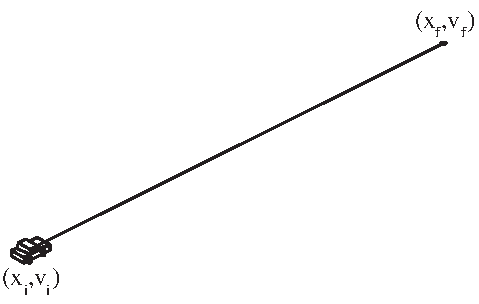
\includegraphics[width=0.6\textwidth]{optimal_control/car_problem_statement}
\caption{Car problem statement.}\label{CarProblemFigure}
\end{center}
\end{figure}
 
 
To simplify the problem, let us approximate the car by a unit point mass
that can be accelerated by using the throttle or decelerated by using the
brake. 
Selecting position and velocity as state variables the mathematical
model of this system becomes a problem of two ordinary differential
equations with their corresponding initial conditions.

The acceleration is bounded by the capability of the engine, and the
deceleration is limited by the braking system parameters. 

As the objective is to make the car reach the final point as quickly as
possible, the objective functional for this problem is given by the final time.

On the other hand, the car is to be driven to a desired position and a
desired velocity. The erros in that target position and velocity are the constraints of the problem.

The statement and the solution itself of this car problem points out a
number of significant issues. First, some variational problems might require
a function space with independent parameters associated to it. Indeed, the
final time is not part of the control, but it represents the interval when it is
defined. Finally, this kind of applications demand spaces of functions with
very good approximation properties, since they are likely to have very non-
linear solutions. Here the optimal control even exhibits discontinuities.


\subsection*{Car problem neurocomputing}

This problem is very similar to the one above. 
It can be formulated as an optimal control problem with one control and two state variables, 
and where the control is subject to two boundary conditions and lower and upper bounds. 
The performance functional has one constraint and requires the integration of a system of two ordinary differential equations. 

Therefore, there main differences between these two car problems are in the number of control variables and in the characteristics of them.
In the problem above the number of control variables is two (acceleration and deceleration), while that in this problem there is just one (acceleration, which can be negative to represent deceleration).
On the other hand, in the problems above, the variables are not subject to any condition,while here the acceleration must be zero at both the initial and final times.

\subsection*{Fed batch fermenter}

The fed batch fermenter problem formulated in this section is an optimal
control problem with one control and four state variables, and defined by
a performance functional with one constraint and requiring the integration
of a system of ordinary differential equations. 

In many biochemical processes, the reactors are operated in fed batch mode,
where the feed rate into the reactor is used for control. 
There is no outflow, so the feed rate must be chosen so that that batch volume does not exceed
the physical volume of the reactor.
As a specific example, an optimization study of the fed batch fermentation
for ethanol production by Saccharomyces cerevisiae is presented.
Figure \ref{EthanolPlantFigure}, taken from Wikipedia, is a picture of a ethanol plant. 

\begin{figure}[!hbp]
\begin{center}
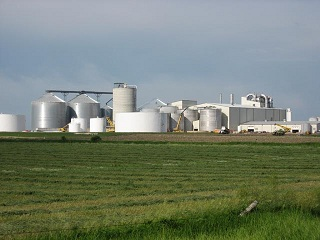
\includegraphics[width=0.7\textwidth]{optimal_control/ethanol_plant}
\caption{Chemical plant for ethanol production.}\label{EthanolPlantFigure}
\end{center}
\end{figure}


The fed batch fermentation process considered here is a process in which
ethanol is produced by Saccharomyces cerevisiae and the production of ethanol
is inhibited by itself.

A batch fermenter generally consists of a closed vessel provided with a
means of stirring and with temperature control. It may be held at constant
pressure or it can be entirely enclosed at a constant volume. In many biochemical processes, 
the reactors are operated in fed batch mode, where the
feed rate into the reactor chosen so that that batch volume does not exceed
the physical volume of the reactor \cite{Luus1993}. 

The states of the plant are the concentration of cell mass, the concentration of substrate, 
the concentration of product and the broth volume in the fermenter. 
The control variable is the feeding rate, and it is
is the only manipulated variable of this process \cite{Luus1993}. 

The dynamic behavior of this fed batch fermentation process can be described by four differential-algebraic equations,
together with their initial conditions. 

The liquid volume of the reactor is limited by the vessel size. This
constraint on the state of the system can be written as an error functional.

The desired objective is to obtain a maximum amount of yield at the end of
the process. The actual yield in the reactor is given by the concentration of
product multiplied by the broth volume in the reactor. 

Since the equations describing the fermenter are nonlinear and the inputs
and states are constrained, the determination of the feed rate to maximize
the yield can be quite difficult.


\subsection*{Aircraft landing}

This is an optimal control problem of aeronautical engineering interest, with one control and
four state variables, and where the objective functional is evaluated by integrating a system of
four ordinary differential equations.

The landing of an aircraft consists of two main stages: the
glide-path phase and the flare-out phase. Here we seek to determine the optimal control and the
corresponding optimal trajectory of an aircraft during its final
approach before landing. 
Figure \ref{AircraftLandingFigure} illustrates the landing process of an aircraft. 
That picture is taken from Wikipedia. 

\begin{figure}[!hbp]
\begin{center}
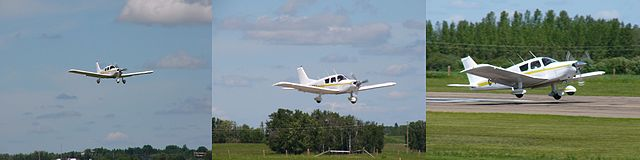
\includegraphics[width=1.0\textwidth]{optimal_control/aircraft_landing}
\caption{Landing of an aircraft.}\label{AircraftLandingFigure}
\end{center}
\end{figure}

The aircraft landing problem examined here is similar to that considered in \cite{Ellert1963}.

In the flare-out phase the longitudinal dynamics of the aircraft
are governed by the pitch angle, which in turn is controlled by the elevator deflection angle \cite{Ashley1992}. 


Figure \ref{AircraftAngles} depicts the
pitch and the elevator deflection angles of an aircraft.

\begin{figure}[h!]
\begin{center}
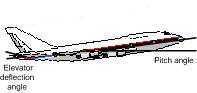
\includegraphics[width=0.5\textwidth]{optimal_control/aircraft_angles.jpg}
\caption{Elevator deflection angle and pitch angle.}\label{AircraftAngles}
\end{center}
\end{figure}

Thus the aim of the aircraft landing problem considered here is to
determine an optimal elevator deflection angle as a function of
time that satisfies a set of performance requirements.

As stated earlier, the elevator controls the longitudinal motion
of the aircraft. It is assumed that any control signal is
instantaneously represented by the elevator. The elevator
deflection angle is also physically limited to a finite range.

The following variables will be used to describe the dynamics of the aircraft \cite{Ellert1963}:
the pitch angle rate, the pitch angle, the altitude rate and, the altitude. 

The velocity of the aircraft and it is assumed to be constant during the flare-out phase. 

The mathematical model shows that the elevator deflection angle
has a direct effect on the pitch angle rate,
which in turn affects the pitch angle, the altitude
rate and the altitude.

The performance requirements define the physical constraints and
desired values of the control and the state variables. The most
important requirements and constraints for the landing system
considered in this problem are highlighted in the following section.

In our example problem the flare-out procedure ends at the final or touchdown time. 

During a process it is often desirable to be able to define the
desired value of a given state variable; this information can then
be used to evaluate the performance of the system. The desired
altitude of the aircraft is the most visual characteristic of the
landing procedure. For this problem it is given by Figure
\ref{DesiredAltitudeFigure}.

\begin{figure}[h!]
\begin{center}
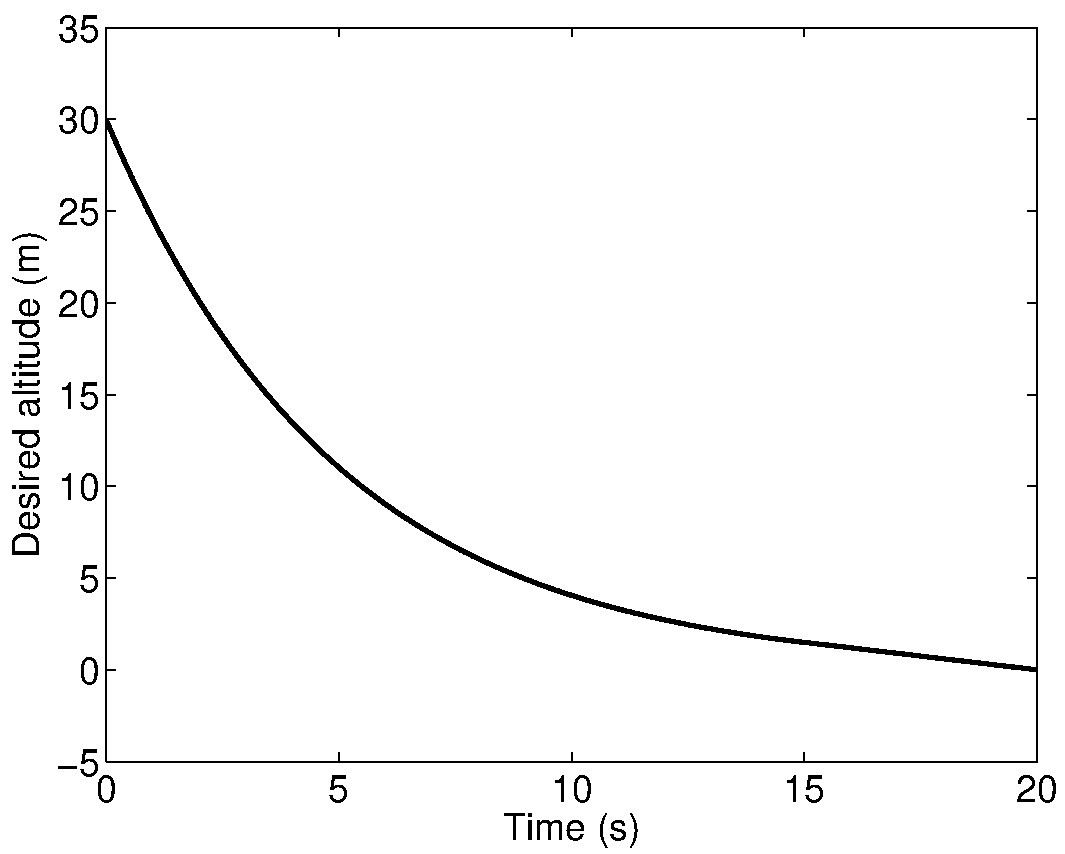
\includegraphics[width=0.6\textwidth]{optimal_control/target_altitude_aircraft_landing}
\caption{Desired landing altitude.}\label{DesiredAltitudeFigure}
\end{center}
\end{figure}

It is desirable to land without expending excessive amounts of
control effort. Therefore, a regularization term can be added. 

At the time of touchdown the pitch angle of the aircraft must lie
in an appropriate range. This requirement is
defined by a set of physical limitations. The lower limit serves
to ensure the nose wheel of a tricycle landing gear does not
touchdown prematurely. Similarly the upper limit is set to prevent
the tail gear touching downing first. A desired pitch angle at
touchdown could be specified as a constraints term. 




